\section{Exigences fonctionnelles des protections}
Cette section a pour but de détailler les différentes exigences que les deux protections vont devoir remplir.

Les protections :
\begin{enumerate}
    \item assureront une protection complète contre les réflexions du laser, afin de garantir la sécurité des utilisateurs du kit.
    \item ne devront pas restreindre l'accessibilité des autres composants, tels que les lentilles réglables ainsi que le laser, afin de pouvoir régler ceux-ci facilement, si nécessaire.
    \item seront des assemblages mécaniques simples à monter et à démonter.
    \item auront une conception simple, afin que leur fabrication soit la plus aisée possible.
    \item comprendront le moins de pièces et de visseries possible.
\end{enumerate}

\section{Protection à l'entrée du laser}
Cette section va expliquer les différentes étapes de la conception de la protection, la modélisation de celle-ci, les prototypes qui ont été réalisés, la fabrication final ainsi que le montage.
\subsection{Prototype initial en carton}
Lorsqu'il est possible de faire un prototype en carton, je le fais afin d'avoir une première idée concrète du projet à réaliser. Ses avantages résident dans le fait que c'est rapide à créer et simple. La première idée a direct été une boîte qui entoure la cage de lentille avec un système de capot qui peut se soulever. Ci-dessous, deux photos du prototype en carton, avec une photo où le capot est fermée, voir Figure \ref{carton_protection_fermee}, et l'autre photo quand la protection est ouverte, voir Figure \ref{carton_protection_ouverte}.

\begin{minipage}[c]{0.48\textwidth}
    \begin{center}
        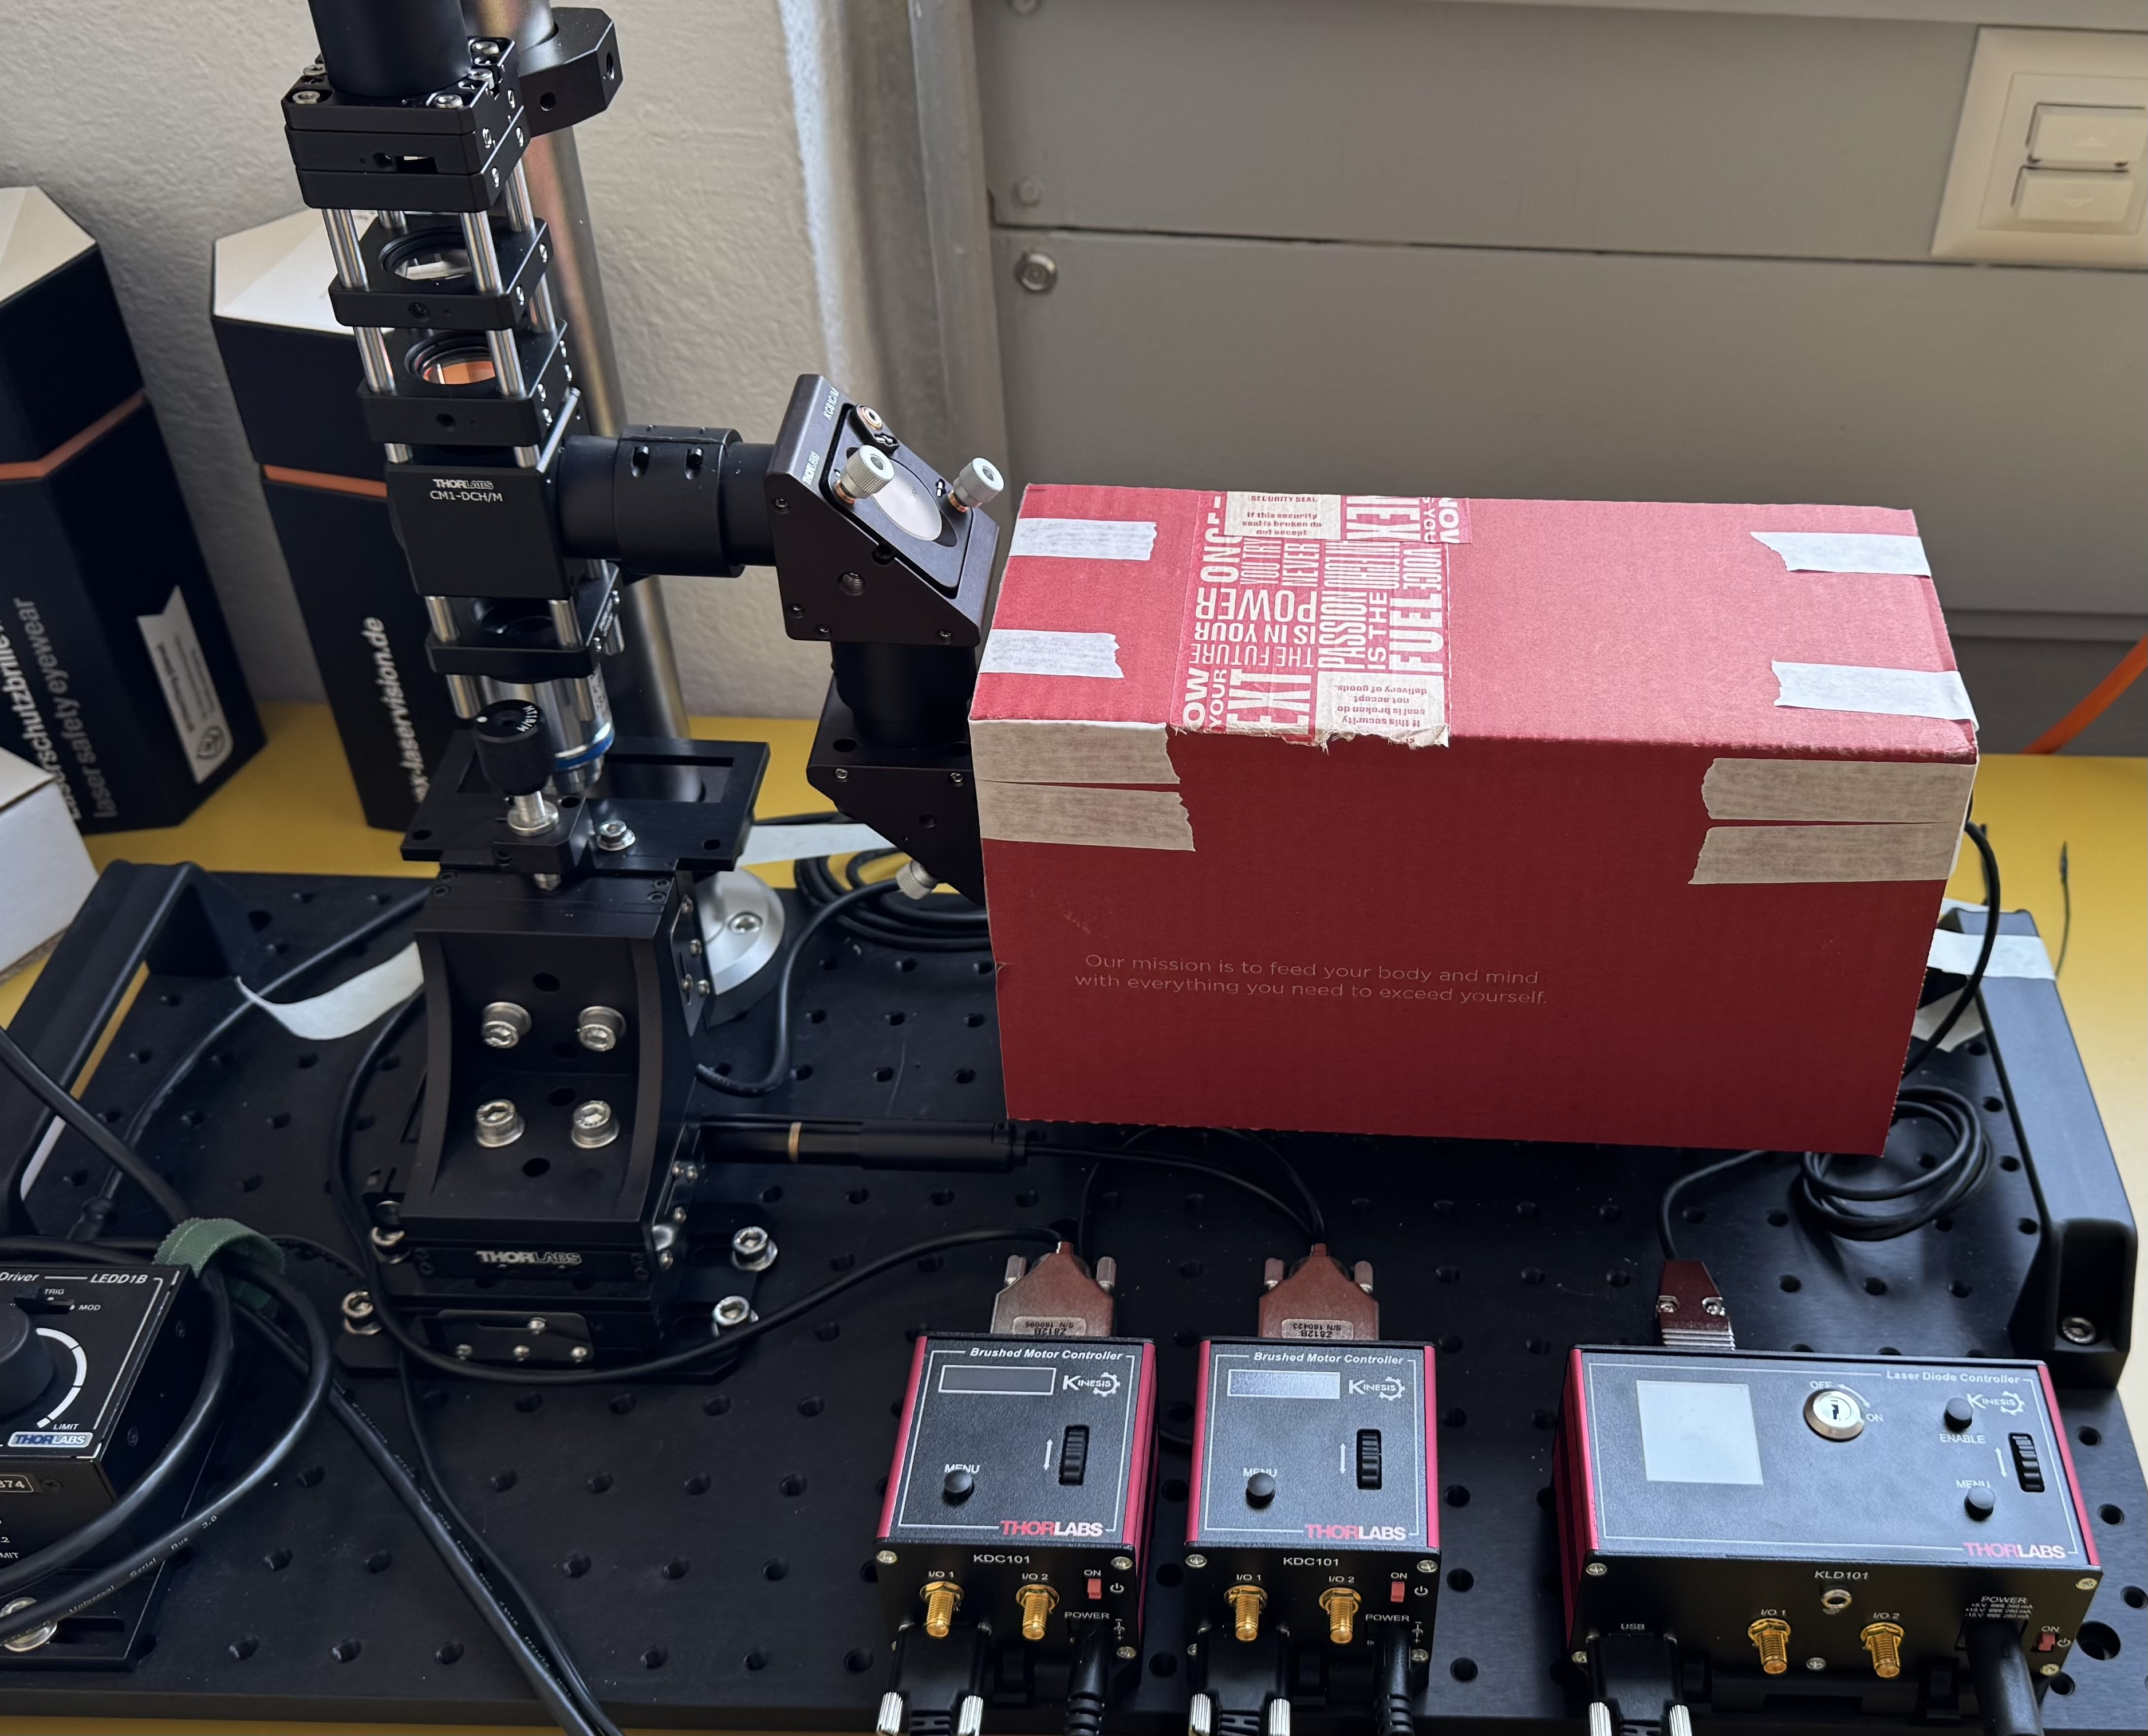
\includegraphics[width=\textwidth]{assets/figures/Protections_laser/Securite_mecanique/Protection_entree_laser/carton_protection_ferme.jpeg}
    \end{center}
    \captionof{figure}{Prototype en carton, protection fermée}
    \label{carton_protection_fermee}
\end{minipage}\hfill
\begin{minipage}[c]{0.48\textwidth}
    \begin{center}
        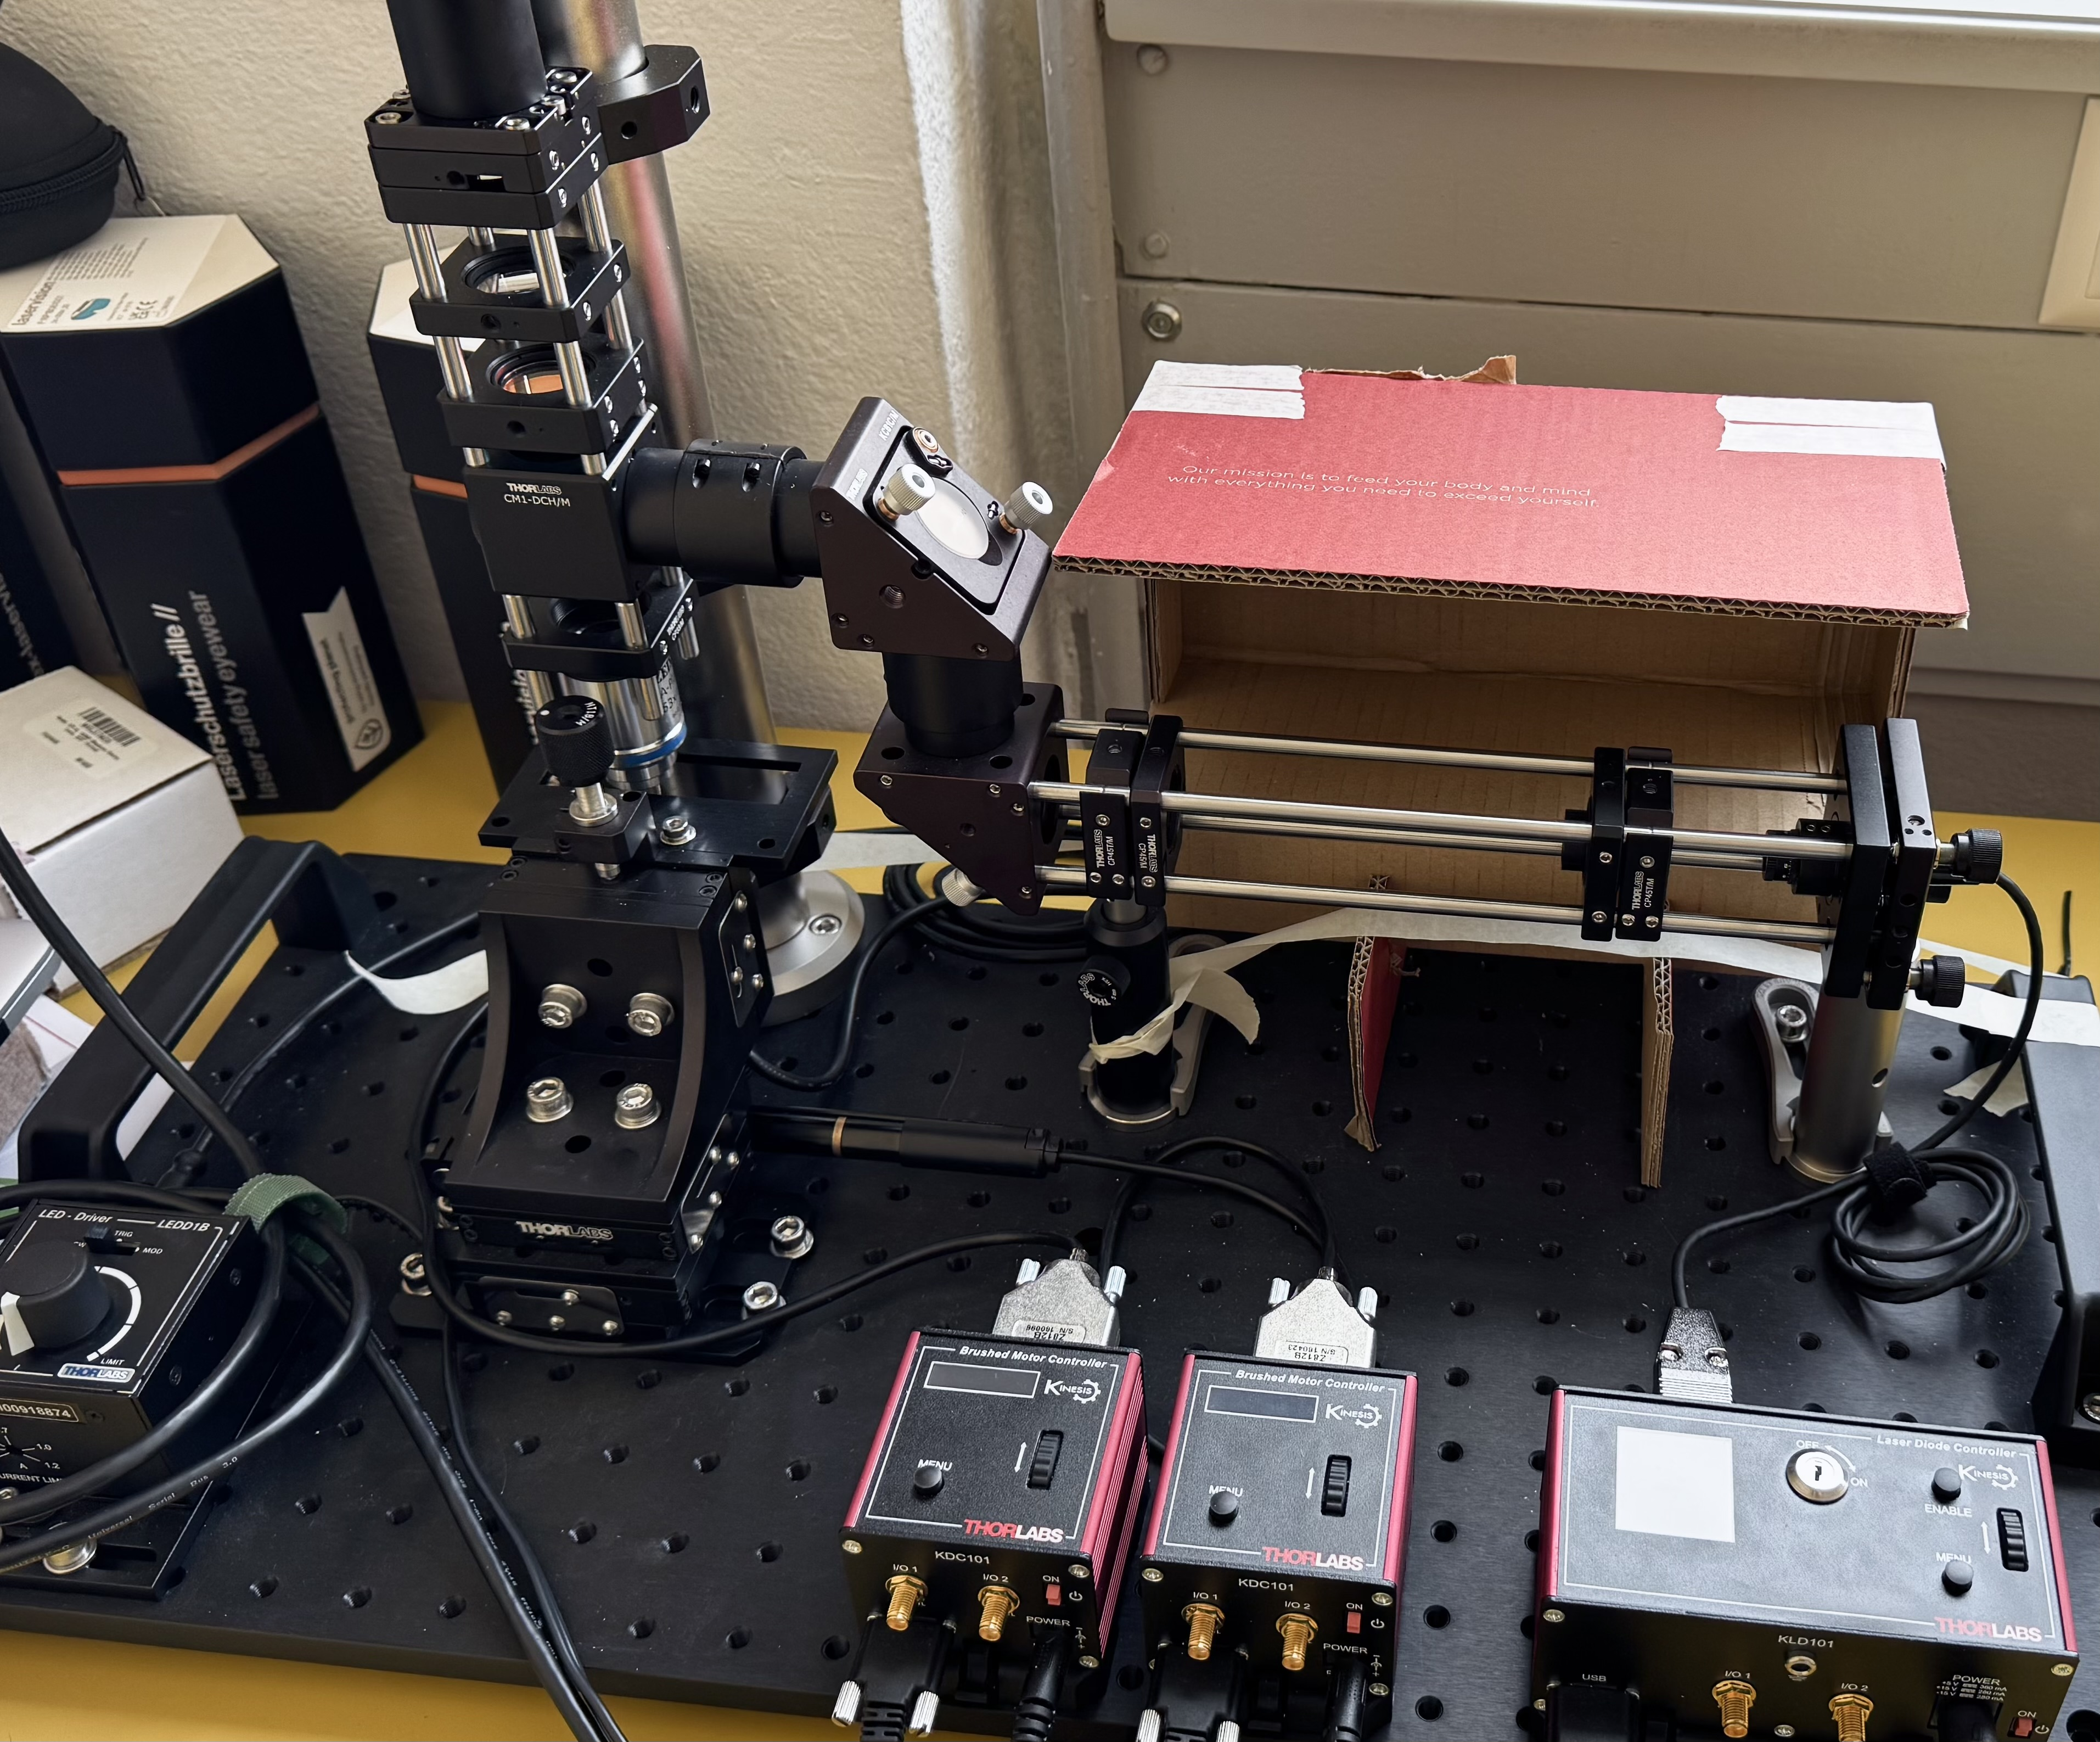
\includegraphics[width=\textwidth]{assets/figures/Protections_laser/Securite_mecanique/Protection_entree_laser/carton_protection_ouvert.jpeg}
    \end{center}
    \captionof{figure}{Prototype en carton, protection ouverte}
    \label{carton_protection_ouverte}
\end{minipage}

\subsection{Modélisation de la protection}
Maintenant que l'idée principale est là, il faut passer à la modélisation de la protection. Avant cette étape, la représentation en 3D du kit complet a été faite, comme expliqué à la page~\pageref{modelisation_3D} au premier paragraphe. Le 3D du kit permet de pouvoir créer la protection en tenant compte de  toutes les contraintes liés aux autres composants, sans devoir faire des mesures sur le kit réel.

Pour pouvoir mieux comprendre les choix de conception et les étapes faites pour réaliser la protection, les Figures~\ref{model_3D_ferme}~et~\ref{model_3D_ouvert}, ci-dessous, représente la modélisation complète de la protection ouverte et fermée.

\begin{minipage}[c]{0.48\textwidth}
    \begin{center}
        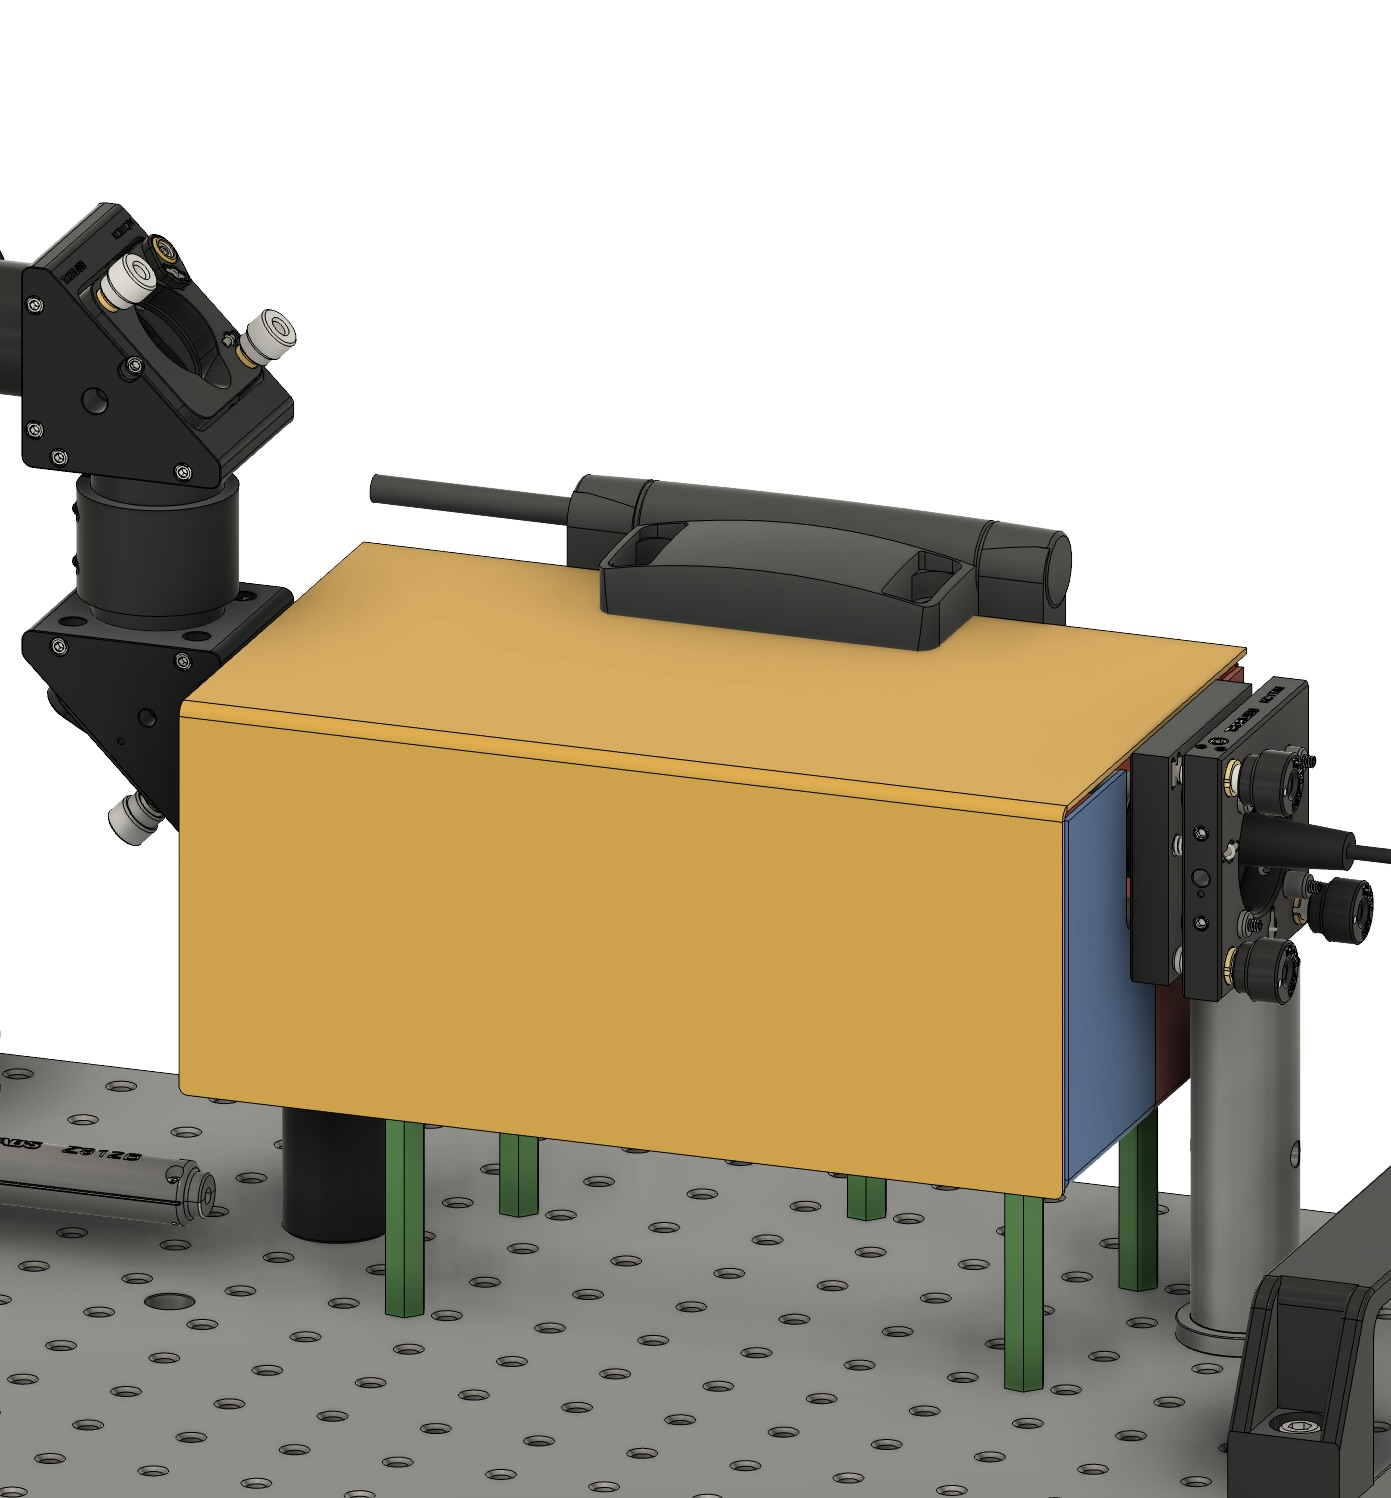
\includegraphics[width=\textwidth]{assets/figures/Protections_laser/Securite_mecanique/Protection_entree_laser/model_3D_ferme.jpeg}
    \end{center}
    \captionof{figure}{Modèle 3D de la protection ouverte}
    \label{model_3D_ferme}
\end{minipage}\hfill
\begin{minipage}[c]{0.48\textwidth}
    \begin{center}
        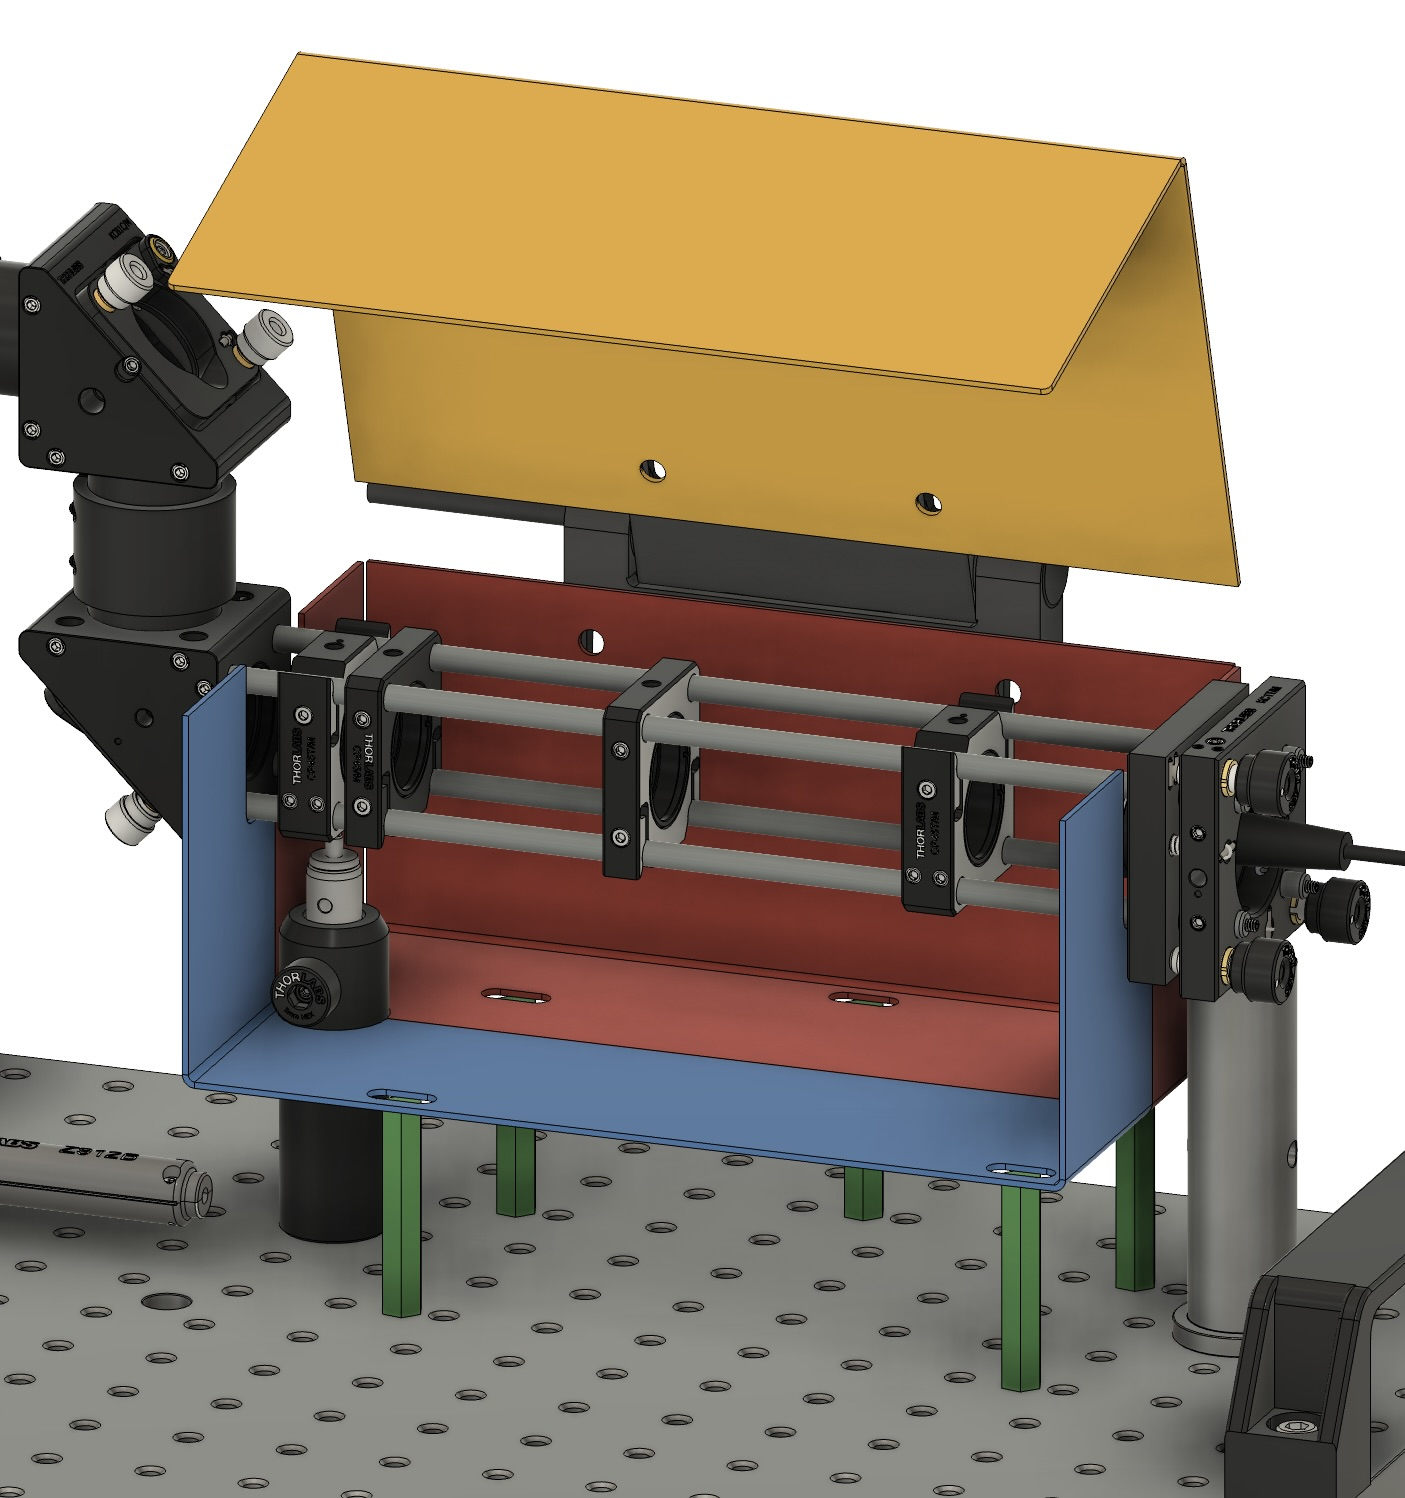
\includegraphics[width=\textwidth]{assets/figures/Protections_laser/Securite_mecanique/Protection_entree_laser/model_3D_ouvert.jpeg}
    \end{center}
    \captionof{figure}{Modèle 3D de la protection fermée}
    \label{model_3D_ouvert}
\end{minipage}

\begin{table}[H]
    \centering
    \caption{Nomenclature des pièces modélisées avec code couleur}
    \begin{tabular}{|c|l|}
        \hline
        \textbf{Couleur}                           & \textbf{Nom de la pièce}                    \\
        \hline
        \textcolor[RGB]{88, 122, 163}{Bleu}        & Capot inférieur avant                       \\
        \textcolor[RGB]{170, 80, 70}{Rouge}        & Capot inférieur arrière                     \\
        \textcolor[RGB]{233, 173, 56}{Jaune}       & Capot supérieur                             \\
        \textcolor[RGB]{100, 100, 100}{Gris foncé} & Charnière reliant les capots inférieurs     \\
        \textcolor[RGB]{70, 170, 70}{Vert}         & Entretoises suportant les capots inférieurs \\
        \hline
    \end{tabular}
    \label{tab:nomenclature_pieces}
\end{table}

\subsubsection{Contraintes rencontrées}

\begin{minipage}[c]{0.4\textwidth}
    La première contrainte a été cet axe noir vertical que l'on voit par la flèche noir sur la Figure~\ref{contrainte_axe_vertical} qui passent à travers les deux capots inférieurs.

    La solution s'est résumé à séparer le capot inférieur en deux, pour pouvoir assembler facilement sans devoir démonter des pièces du kit original.
\end{minipage}\hfill
\begin{minipage}[c]{0.58\textwidth}
    \begin{center}
        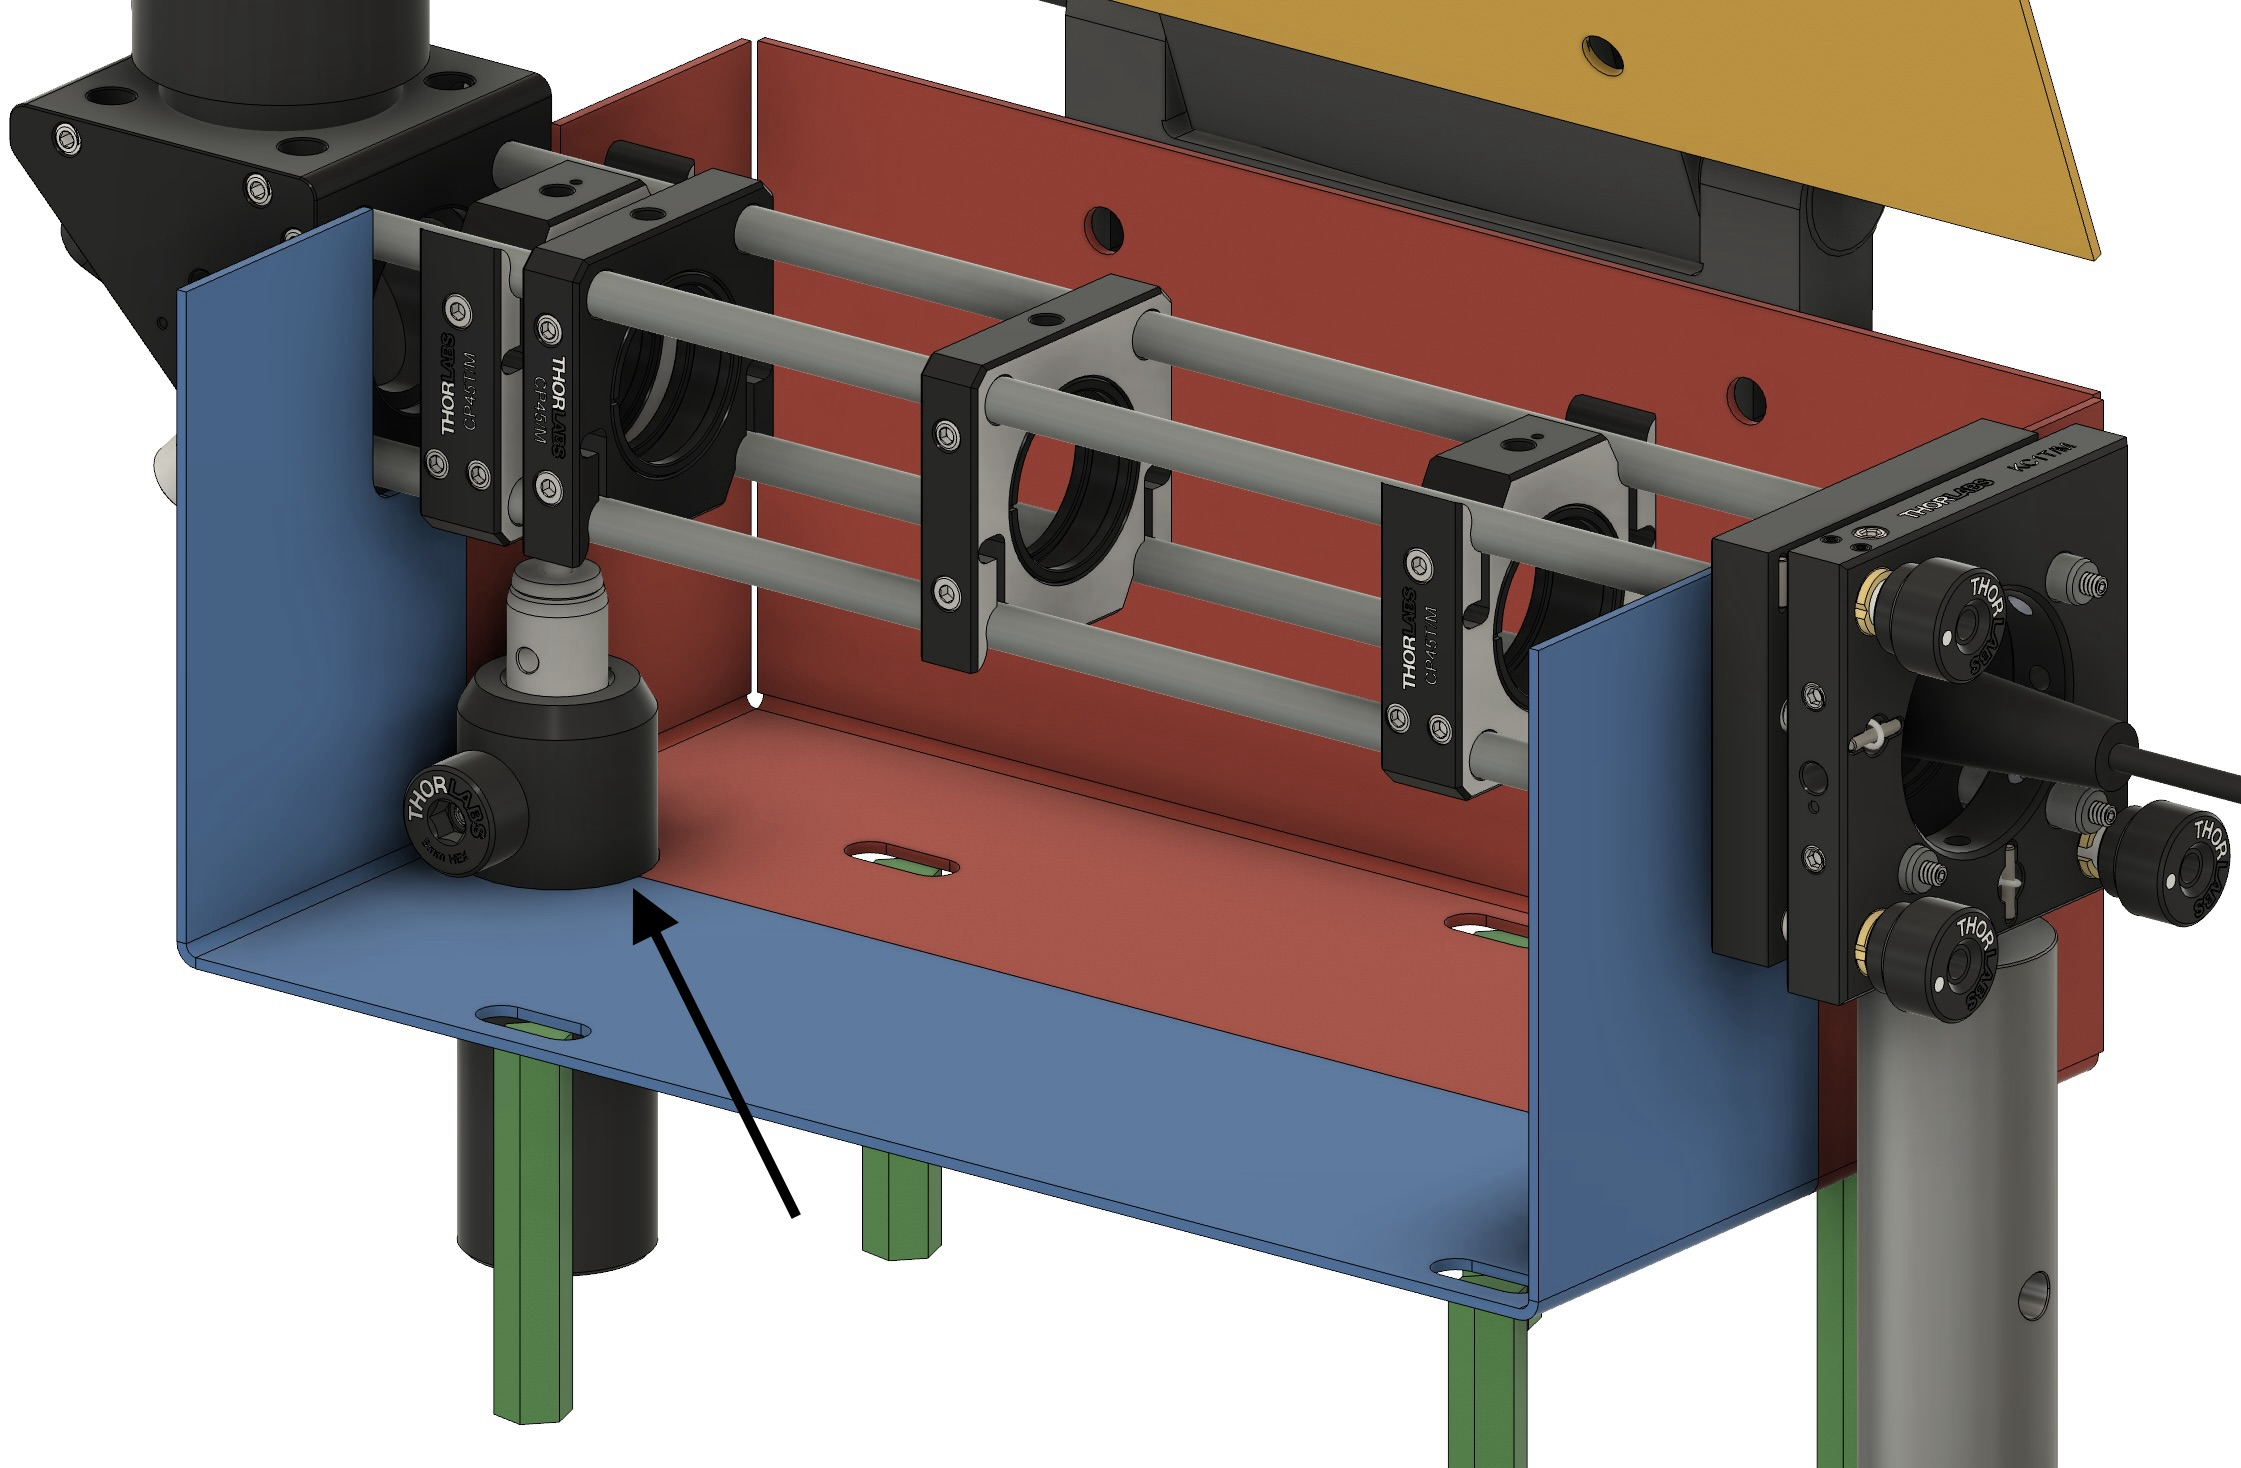
\includegraphics[width=\textwidth]{assets/figures/Protections_laser/Securite_mecanique/Protection_entree_laser/contrainte_axe_vertical.jpeg}
    \end{center}
    \captionof{figure}{Axe vertical traversant les protections inférieures}
    \label{contrainte_axe_vertical}
\end{minipage}

\begin{minipage}[c]{0.4\textwidth}
    Une contrainte supplémentaire a été cette vis de réglage indiquée par la flèche noir sur la Figure~\ref{contrainte_vis}. Elle se situe dans la course du capot supérieur.

    La solution retenue a été de s'assurer que toutes les protections, dans le plan horizontal, ne dépassent pas la largeur de la vis. Cette contrainte en entraîne une autre, qui sera détaillée ensuite.
\end{minipage}\hfill
\begin{minipage}[c]{0.58\textwidth}
    \begin{center}
        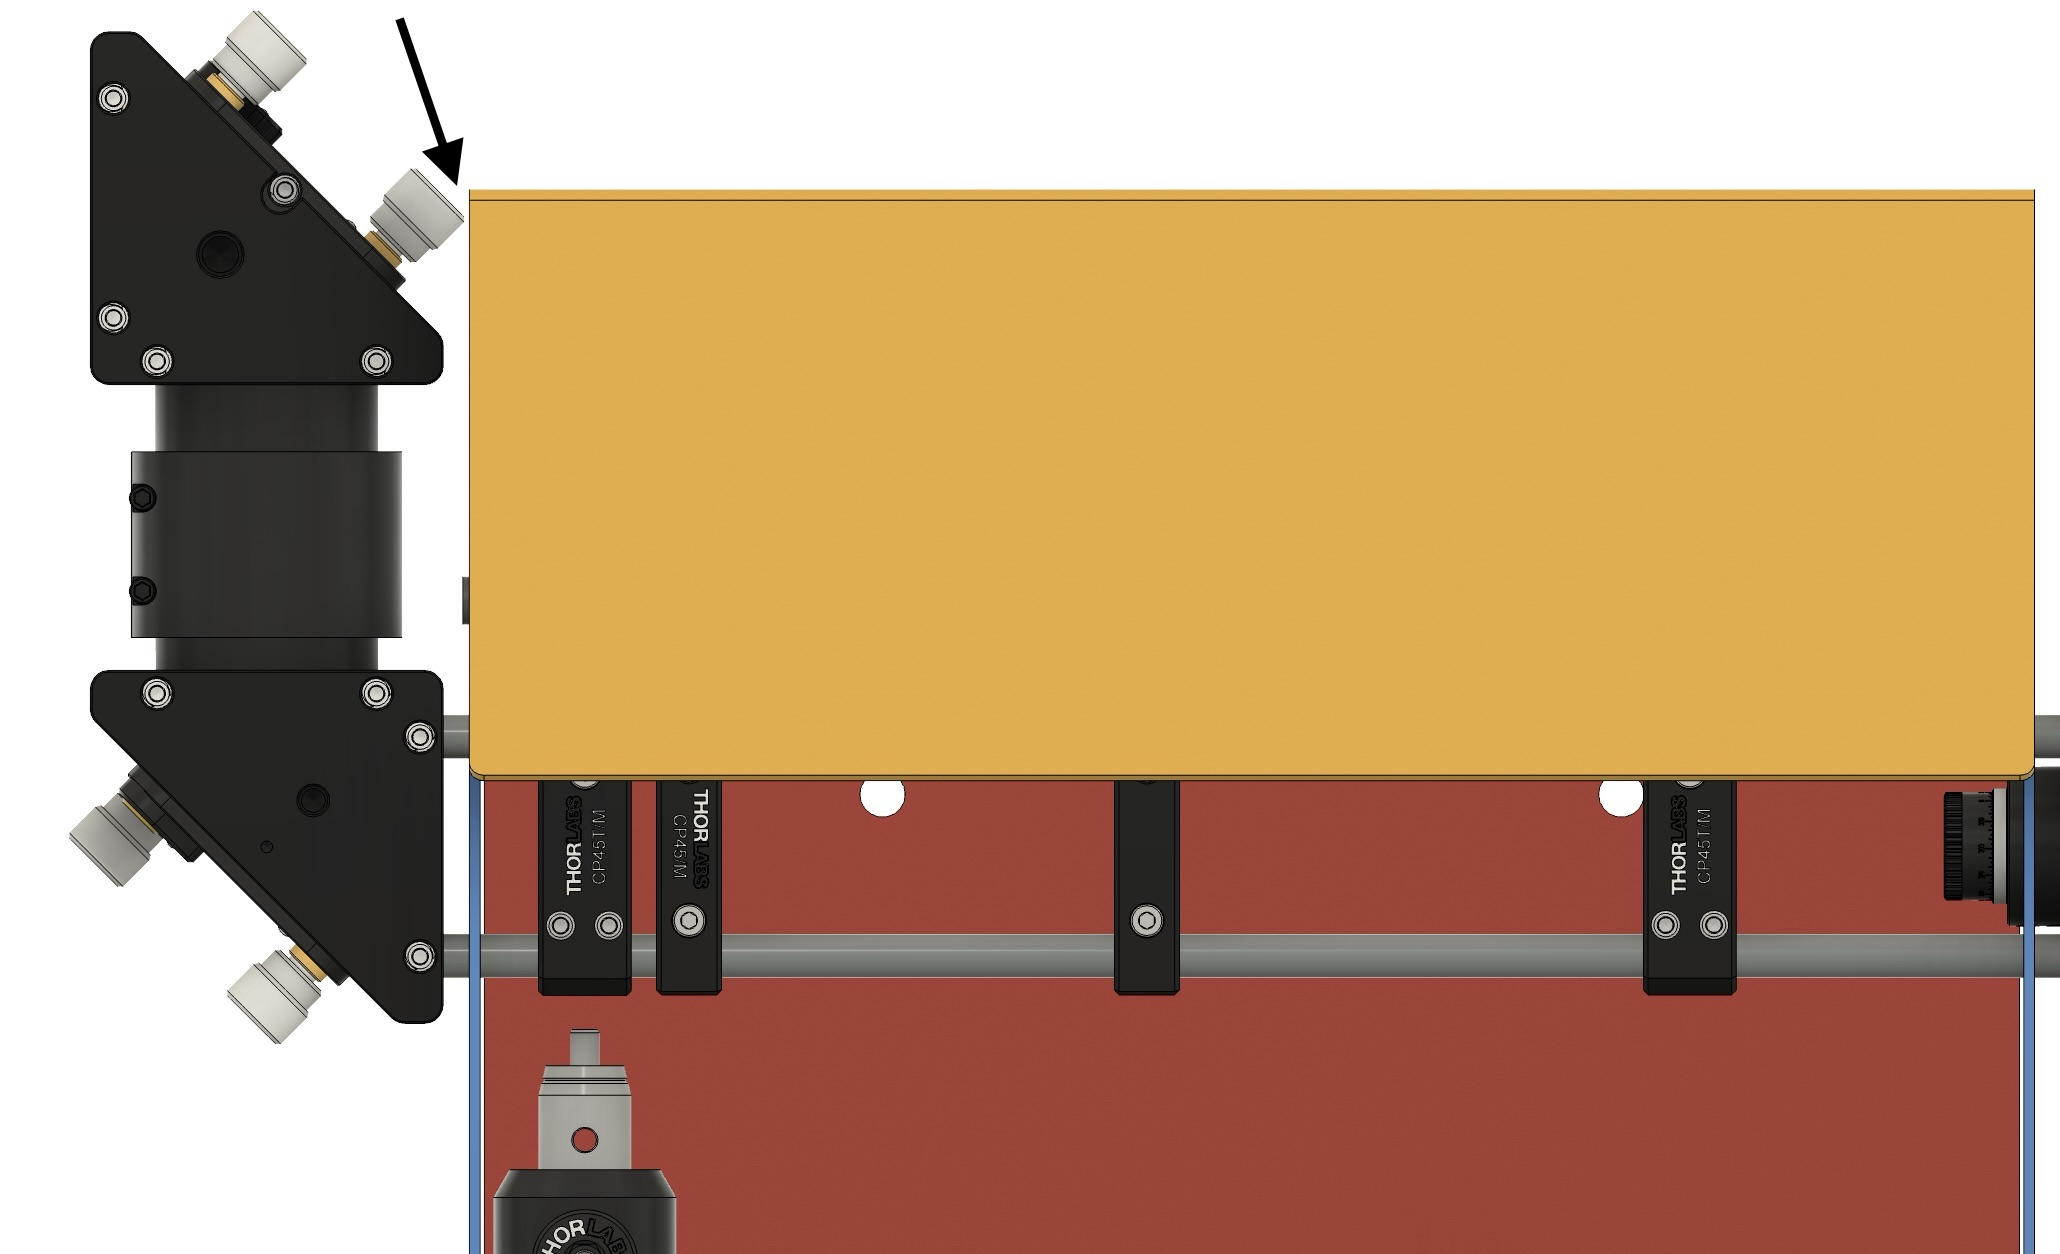
\includegraphics[width=\textwidth]{assets/figures/Protections_laser/Securite_mecanique/Protection_entree_laser/contrainte_vis.jpeg}
    \end{center}
    \captionof{figure}{Vis de réglage dans la course du capot supérieur}
    \label{contrainte_vis}
\end{minipage}

\begin{minipage}[c]{0.5\textwidth}
    La contrainte qui découle de la vis de réglage, et vu l'obligation de réduire la taille des protections, cela a créer un vide pouvant laisser passer les rayons du laser. Les traits manuscrits en rouge sur la Figure~\ref{contrainte_passage_laser_cage} représentent les fuites potentielles du laser. Ce phénomène apparaît également à droite des protections.

    La solution apportée a été d'ajouter un joint en mousse souple entourant les quatres axes qui formant la cage. Les protections viendraient s'appuyer sur les joints et combleraient les vides. Les détails en photo pour cette solution sont montrés à la section~\ref{prototype_bois}.
\end{minipage}\hfill
\begin{minipage}[c]{0.48\textwidth}
    \begin{center}
        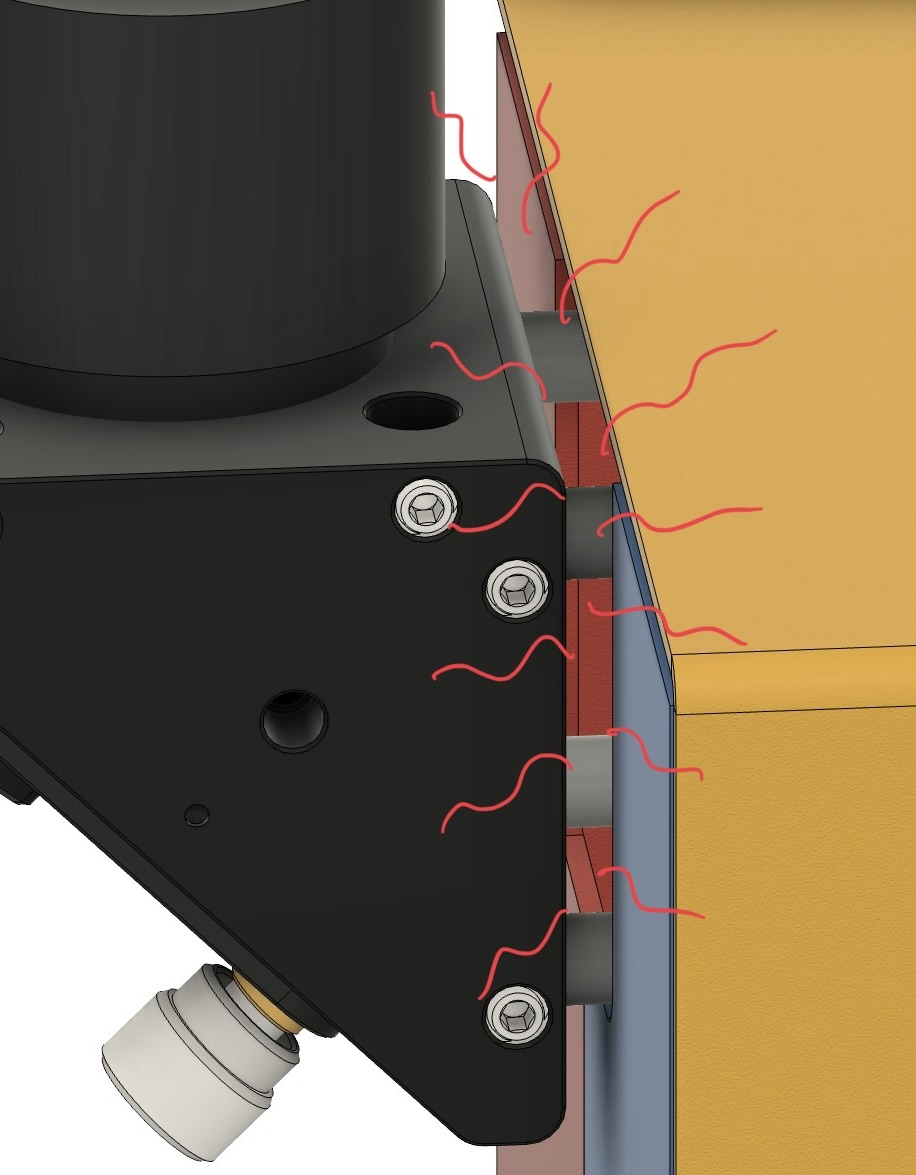
\includegraphics[width=0.9\textwidth]{assets/figures/Protections_laser/Securite_mecanique/Protection_entree_laser/contrainte_passage_laser_cage.jpeg}
    \end{center}
    \captionof{figure}{Fuites potentielles des rayons du laser}
    \label{contrainte_passage_laser_cage}
\end{minipage}

\begin{minipage}[c]{0.6\textwidth}
    La dernière contrainte est similaire à la précédente, car elle aussi vient contrer les fuites possibles du laser. Cependant, cette fois c'est pour la protection supérieure. En effet, lorsque le capot est fermé, il y'a un risque qu'il y ait des espaces fins où la lumière du faisceau peut s'échapper.

    La solution va également être la pose d'un joint, cette fois à l'intérieur du capot supérieur sur tout son contour. Ainsi, lorsque la protection est fermée, le joint va combler les vides. La modélisation ci-contre, voir la Figure~\ref{contrainte_passage_laser_capot}, montre qu'un espace entre la partie inférieure est supérieur de la protection a volontairement été créer afin de laisser de la place pour le joint.

    La solution apportée a été d'ajouter un joint en mousse souple entourant les quatres axes qui formant la cage. Les protections viendraient s'appuyer sur les joints et combleraient les vides. Les détails en photo pour cette solution sont montrés à la section~\ref{prototype_bois}.
\end{minipage}\hfill
\begin{minipage}[c]{0.38\textwidth}
    \begin{center}
        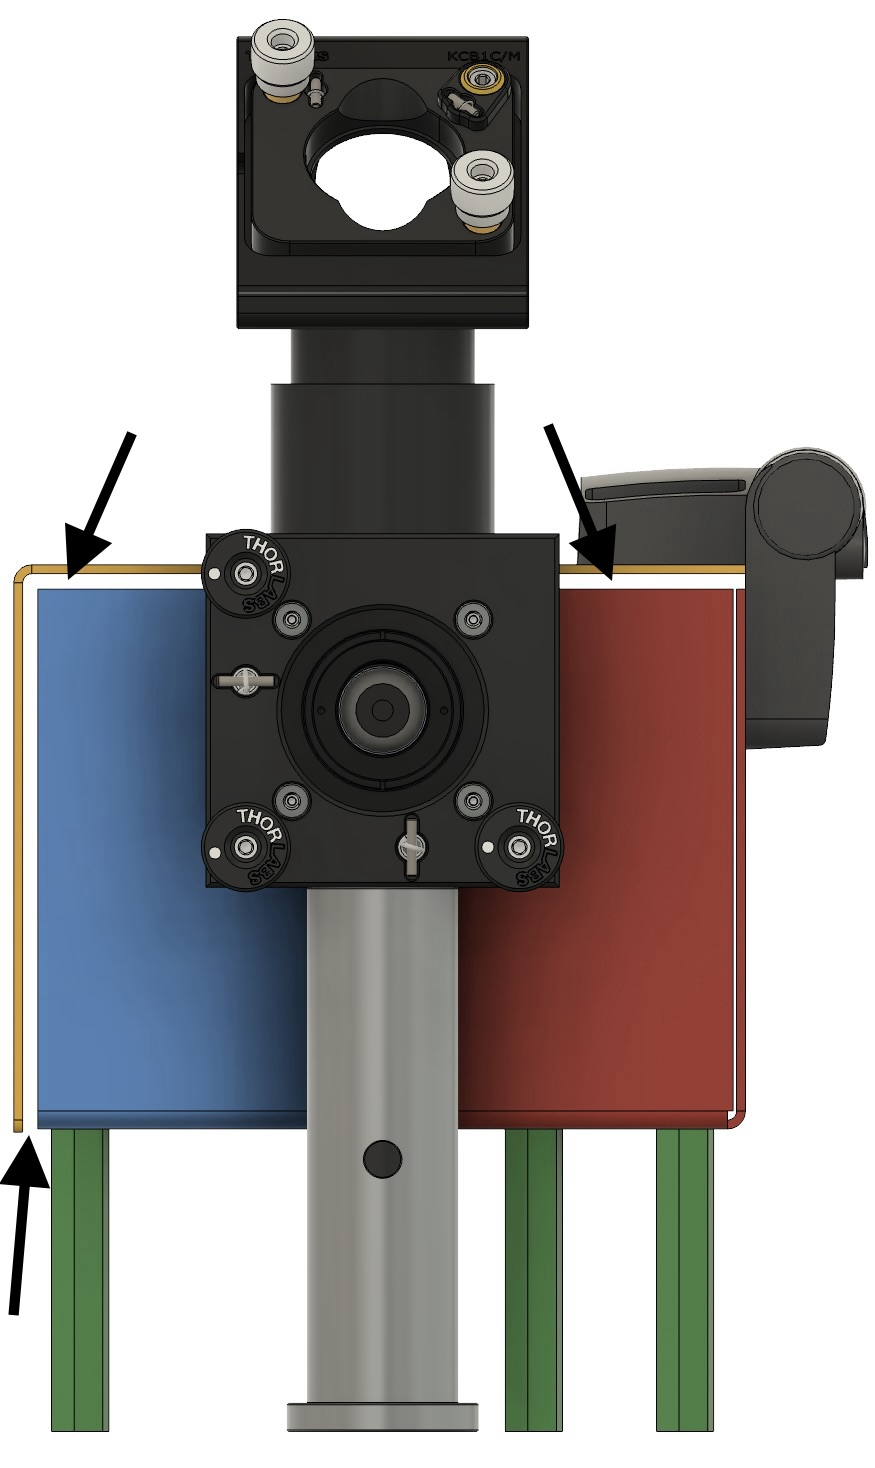
\includegraphics[width=\textwidth]{assets/figures/Protections_laser/Securite_mecanique/Protection_entree_laser/contrainte_passage_laser_capot.jpeg}
    \end{center}
    \captionof{figure}{Fuites potentielles des rayons du laser}
    \label{contrainte_passage_laser_capot}
\end{minipage}

\subsection{Réalisation d'un prototype en bois} \label{prototype_bois}
Une fois la protection modélisée, j'ai réalisé les trois pièces en bois d'épaisseur 3~mm, afin d'être sur des dimensions des pièces.

\subsection{Fabrication des pièces en aluminium}

\subsection{Montage final et ajustements}

\subsection{Intégration de la protection dans le système}

\subsection{Points d'améliorations}

% \subsection{Compatibilité avec le système optique}

% \subsection{Fonctionnement avec le système d'interlock}

\section{Protection vers le microscope}

